\documentclass[12pt]{article}
\usepackage[utf8]{inputenc}
\usepackage[T1]{fontenc}
\usepackage{geometry}
\geometry{a4paper, margin=2cm}
\usepackage{xcolor}
\usepackage{tikz}
\usetikzlibrary{shapes, arrows.meta, positioning, calc, shadows.blur, backgrounds, fit}
\usepackage[most]{tcolorbox}
\usepackage{fontawesome5}
\usepackage{enumitem}

% Colors
\definecolor{paperBlue}{RGB}{70, 130, 180}
\definecolor{paperRed}{RGB}{205, 92, 92}
\definecolor{paperGreen}{RGB}{60, 179, 113}
\definecolor{loraGold}{RGB}{218, 165, 32}
\definecolor{bgGray}{RGB}{250, 250, 250}
\definecolor{paperPurple}{RGB}{147, 112, 219}

% Environment
\newtcolorbox{casestudy}[2][]{
    enhanced, 
    colback=bgGray!50!white, 
    colframe=paperBlue,
    coltitle=white, 
    title={\textbf{#2}}, 
    fonttitle=\large\sffamily,
    sharp corners, 
    rounded corners=southeast, 
    arc=6mm, 
    drop shadow, 
    #1
}

\newcommand{\score}[1]{\textcolor{paperGreen}{\textbf{#1}}}

\pagestyle{empty}

\begin{document}

% Case A
\begin{casestudy}{Caso A: Usuario de Polonia (Indie Rock / Post-Punk)}
    \begin{minipage}[t]{0.48\textwidth}
        \textbf{\faUser\ Perfil de Entrada:}
        \begin{itemize}
            \item \textbf{Historial (Selección):}
            \begin{enumerate}
                \item \textit{The Killers} - Somebody Told Me
                \item \textit{Arctic Monkeys} - Bigger Boys and Stolen Sweethearts
                \item \textit{Kasabian} - L.S.F.
                \item \textit{Franz Ferdinand} - Take Me Out
                \item \textit{Arctic Monkeys} - When The Sun Goes Down
            \end{enumerate}
            \item \textbf{Contexto:} Polonia
        \end{itemize}
    \end{minipage}
    \hfill
    \begin{minipage}[t]{0.48\textwidth}
        \textbf{\faRobot\ Recomendaciones del Modelo:}
        \begin{enumerate}
            \item \textit{Panic At The Disco} - I Write Sins Not Tragedies \score{0.4859}
            \item \textit{Arctic Monkeys} - A Certain Romance \score{0.4554}
            \item \textit{Arctic Monkeys} - Still Take You Home \score{0.4369}
            \item \textit{Arctic Monkeys} - Red Light Indicates Doors Are Secured \score{0.4362}
            \item \textit{Arctic Monkeys} - Fake Tales Of San Francisco \score{0.4287}
        \end{enumerate}
    \end{minipage}
    
    \vspace{0.3cm}
    \hrule
    \vspace{0.2cm}
    
    \textbf{\faSearch\ Análisis:} el sistema exhibe una \textbf{alta fidelidad secuencial}. La torre de usuario ha identificado el "token" latente de \textit{Arctic Monkeys} como un atractor dominante. Lo notable es el fenómeno de \textit{"Deep Cut"}: recupera \textit{B-sides} y canciones no-singles, sugiriendo que el modelo ha aprendido una representación densa del artista. Prioriza la coherencia de género sobre la diversidad exploratoria.
\end{casestudy}

\newpage

% Case B
\begin{casestudy}[colframe=paperRed]{Caso B: Usuario de México (Nu-Metal vs. Pop Latino)}
    \begin{minipage}[t]{0.48\textwidth}
        \textbf{\faUser\ Perfil de Entrada:}
        \begin{itemize}
            \item \textbf{Historial (Selección):}
            \begin{enumerate}
                \item \textit{Linkin Park} - New Divide
                \item \textit{Angel Y Khriz} - Na De Na
                \item \textit{Nickelback} - How You Remind Me
                \item \textit{Shakira} - Hips Don't Lie (feat. Wyclef Jean)
                \item \textit{Filter} - Take A Picture
            \end{enumerate}
            \item \textbf{Contexto:} México
        \end{itemize}
    \end{minipage}
    \hfill
    \begin{minipage}[t]{0.48\textwidth}
        \textbf{\faRobot\ Recomendaciones del Modelo:}
        \begin{enumerate}
            \item \textit{Belanova} - Tus Ojos \score{0.5717}
            \item \textit{Selena} - Bidi Bidi Bom Bom \score{0.5699}
            \item \textit{Aleks Syntek} - Sexo Pudor Y Lágrimas \score{0.5675}
            \item \textit{Mats Ronander} - Gör mig lycklig nu \score{0.5613}
            \item \textit{Juanes} - Fotografía \score{0.5585}
        \end{enumerate}
    \end{minipage}
    
    \vspace{0.3cm}
    \hrule
    \vspace{0.2cm}
    
    \textbf{\faSearch\ Análisis:} este caso ilustra la \textbf{potencia de los priors demográficos}. El modelo detectó una señal débil de "latinidad" (\textit{Angel Y Khriz}, \textit{Shakira}) y, al combinarla con el embedding explícito de \texttt{Country=Mexico}, colapsó la distribución hacia el clúster regional.
    
    \vspace{0.3cm}
    \begin{center}
    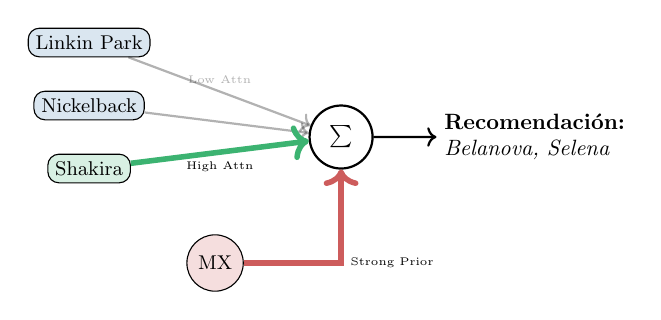
\begin{tikzpicture}[scale=0.8, transform shape]
        % Nodos del historial
        \node[draw, fill=paperBlue!20, rounded corners] (h1) at (0, 2) {\small Linkin Park};
        \node[draw, fill=paperBlue!20, rounded corners] (h2) at (0, 1) {\small Nickelback};
        \node[draw, fill=paperGreen!20, rounded corners] (h3) at (0, 0) {\small Shakira};
        
        % Nodo de contexto
        \node[draw, fill=paperRed!20, circle] (ctx) at (2, -1.5) {\small MX};
        
        % Nodo de atención/fusión
        \node[draw, circle, thick, minimum size=1cm] (attn) at (4, 0.5) {$\sum$};
        
        % Flechas con grosores variables representando atención
        \draw[->, thick, opacity=0.3] (h1) -- node[above, font=\tiny]{Low Attn} (attn);
        \draw[->, thick, opacity=0.3] (h2) -- (attn);
        \draw[->, line width=2pt, paperGreen] (h3) -- node[below, font=\tiny, black]{High Attn} (attn);
        \draw[->, line width=2pt, paperRed] (ctx) -| node[right, font=\tiny, black]{Strong Prior} (attn);
        
        % Output
        \node[right=1cm of attn, align=left] (out) {\textbf{Recomendación:}\\ \textit{Belanova, Selena}};
        \draw[->, thick] (attn) -- (out);
    \end{tikzpicture}
    \end{center}
\end{casestudy}

\newpage

% Case C
\begin{casestudy}[colframe=loraGold]{Caso C: Usuario de China (IDM / Trip-Hop)}
    \begin{minipage}[t]{0.48\textwidth}
        \textbf{\faUser\ Perfil de Entrada:}
        \begin{itemize}
            \item \textbf{Historial (Selección):}
            \begin{enumerate}
                \item \textit{Massive Attack} - Teardrop
                \item \textit{Rage Against The Machine} - Killing In The Name
                \item \textit{Dj Shadow} - Giving Up The Ghost
                \item \textit{Portishead} - Sour Times
                \item \textit{Radiohead} - Fake Plastic Trees
            \end{enumerate}
            \item \textbf{Contexto:} China
        \end{itemize}
    \end{minipage}
    \hfill
    \begin{minipage}[t]{0.48\textwidth}
        \textbf{\faRobot\ Recomendaciones del Modelo:}
        \begin{enumerate}
            \item \textit{Plaid} - Milh \score{0.5081}
            \item \textit{The Future Sound Of London} - Papua New Guinea (Blue States Full Length Mix) \score{0.4949}
            \item \textit{Digitonal} - Wide-Eyed, Wrapped In Love \score{0.4873}
            \item \textit{Casino Versus Japan} - Manic Thru Tone \score{0.4869}
            \item \textit{The Future Sound Of London} - Papua New Guinea (Andrew Weatherall Full Length Mix) \score{0.4858}
        \end{enumerate}
    \end{minipage}
    
    \vspace{0.3cm}
    \hrule
    \vspace{0.2cm}
    
    \textbf{\faSearch\ Análisis:} aquí observamos la verdadera capacidad \textbf{multimodal}. El modelo \textit{ignora} el embedding de país (China) y no recomienda C-Pop. En su lugar, realiza una \textbf{alineación espectral}, recomendando artistas que comparten características acústicas muy específicas (breakbeats lentos, texturas sintéticas) con el historial. La señal de audio "vetó" al sesgo demográfico.
\end{casestudy}

\newpage

% Case D
\begin{casestudy}[colframe=paperPurple]{Caso D: Usuario de Japón (Eclecticismo Vocal)}
    \begin{minipage}[t]{0.48\textwidth}
        \textbf{\faUser\ Perfil de Entrada:}
        \begin{itemize}
            \item \textbf{Historial (Selección):}
            \begin{enumerate}
                \item \textit{Nelly Furtado} - Maneater
                \item \textit{Duffy} - Mercy
                \item \textit{Vetusta Morla} - Copenhague
                \item \textit{Alicia Keys} - If I Ain't Got You
                \item \textit{Elvis Presley} - Suspicious Minds
            \end{enumerate}
            \item \textbf{Contexto:} Japón
        \end{itemize}
    \end{minipage}
    \hfill
    \begin{minipage}[t]{0.48\textwidth}
        \textbf{\faRobot\ Recomendaciones del Modelo:}
        \begin{enumerate}
            \item \textit{Eva Dahlgren} - Ängeln i rummet \score{0.5391}
            \item \textit{Mats Ronander} - Gör mig lycklig nu \score{0.5288}
            \item \textit{Andrea Bocelli} - L'appuntamento (Sentado a 'beira do caminho) \score{0.5196}
            \item \textit{Fiona Apple} - Paper Bag \score{0.5126}
            \item \textit{Andrea Bocelli} - Cuando Me Enamoro \score{0.5113}
        \end{enumerate}
    \end{minipage}
    
    \vspace{0.3cm}
    \hrule
    \vspace{0.2cm}

    \textbf{\faSearch\ Análisis:} este caso demuestra una \textbf{generalización basada en características latentes de audio (Timbre Vocal)} que trasciende el idioma. El modelo detectó un patrón de "Voces Femeninas Melódicas" y recomendó artistas europeas que encajan en ese perfil sonoro. La presencia reciente de \textit{Vetusta Morla} actuó como una "puerta de enlace" hacia idiomas romances/germánicos.
\end{casestudy}

\end{document}